%!TEX root = Thesis_David_Burns.tex

%Todo

% - send to mum for editing
% - send to zoran to check content

%Done

% - Get rough version of totally complete chapter
% - remove all the '' reminders and any quotations
% - put in self referencing
% - prep final draft
% - print and self edit

\chapter{The Great Barrier Reef}
\label{ch:gbr}

	The Great Barrier Reef (\gls{gbr}) is the world's largest organic structure. The marine park encompassing it is \SI{344400}{\square\km} (see \cref{fig:gbrboundary}), of which around \SI{6}{\percent} is comprised of \SI{2900}{} separate coral reefs \citep{borthwick:2006uv}.

	\begin{figure}[!htb]
	    \centering
	    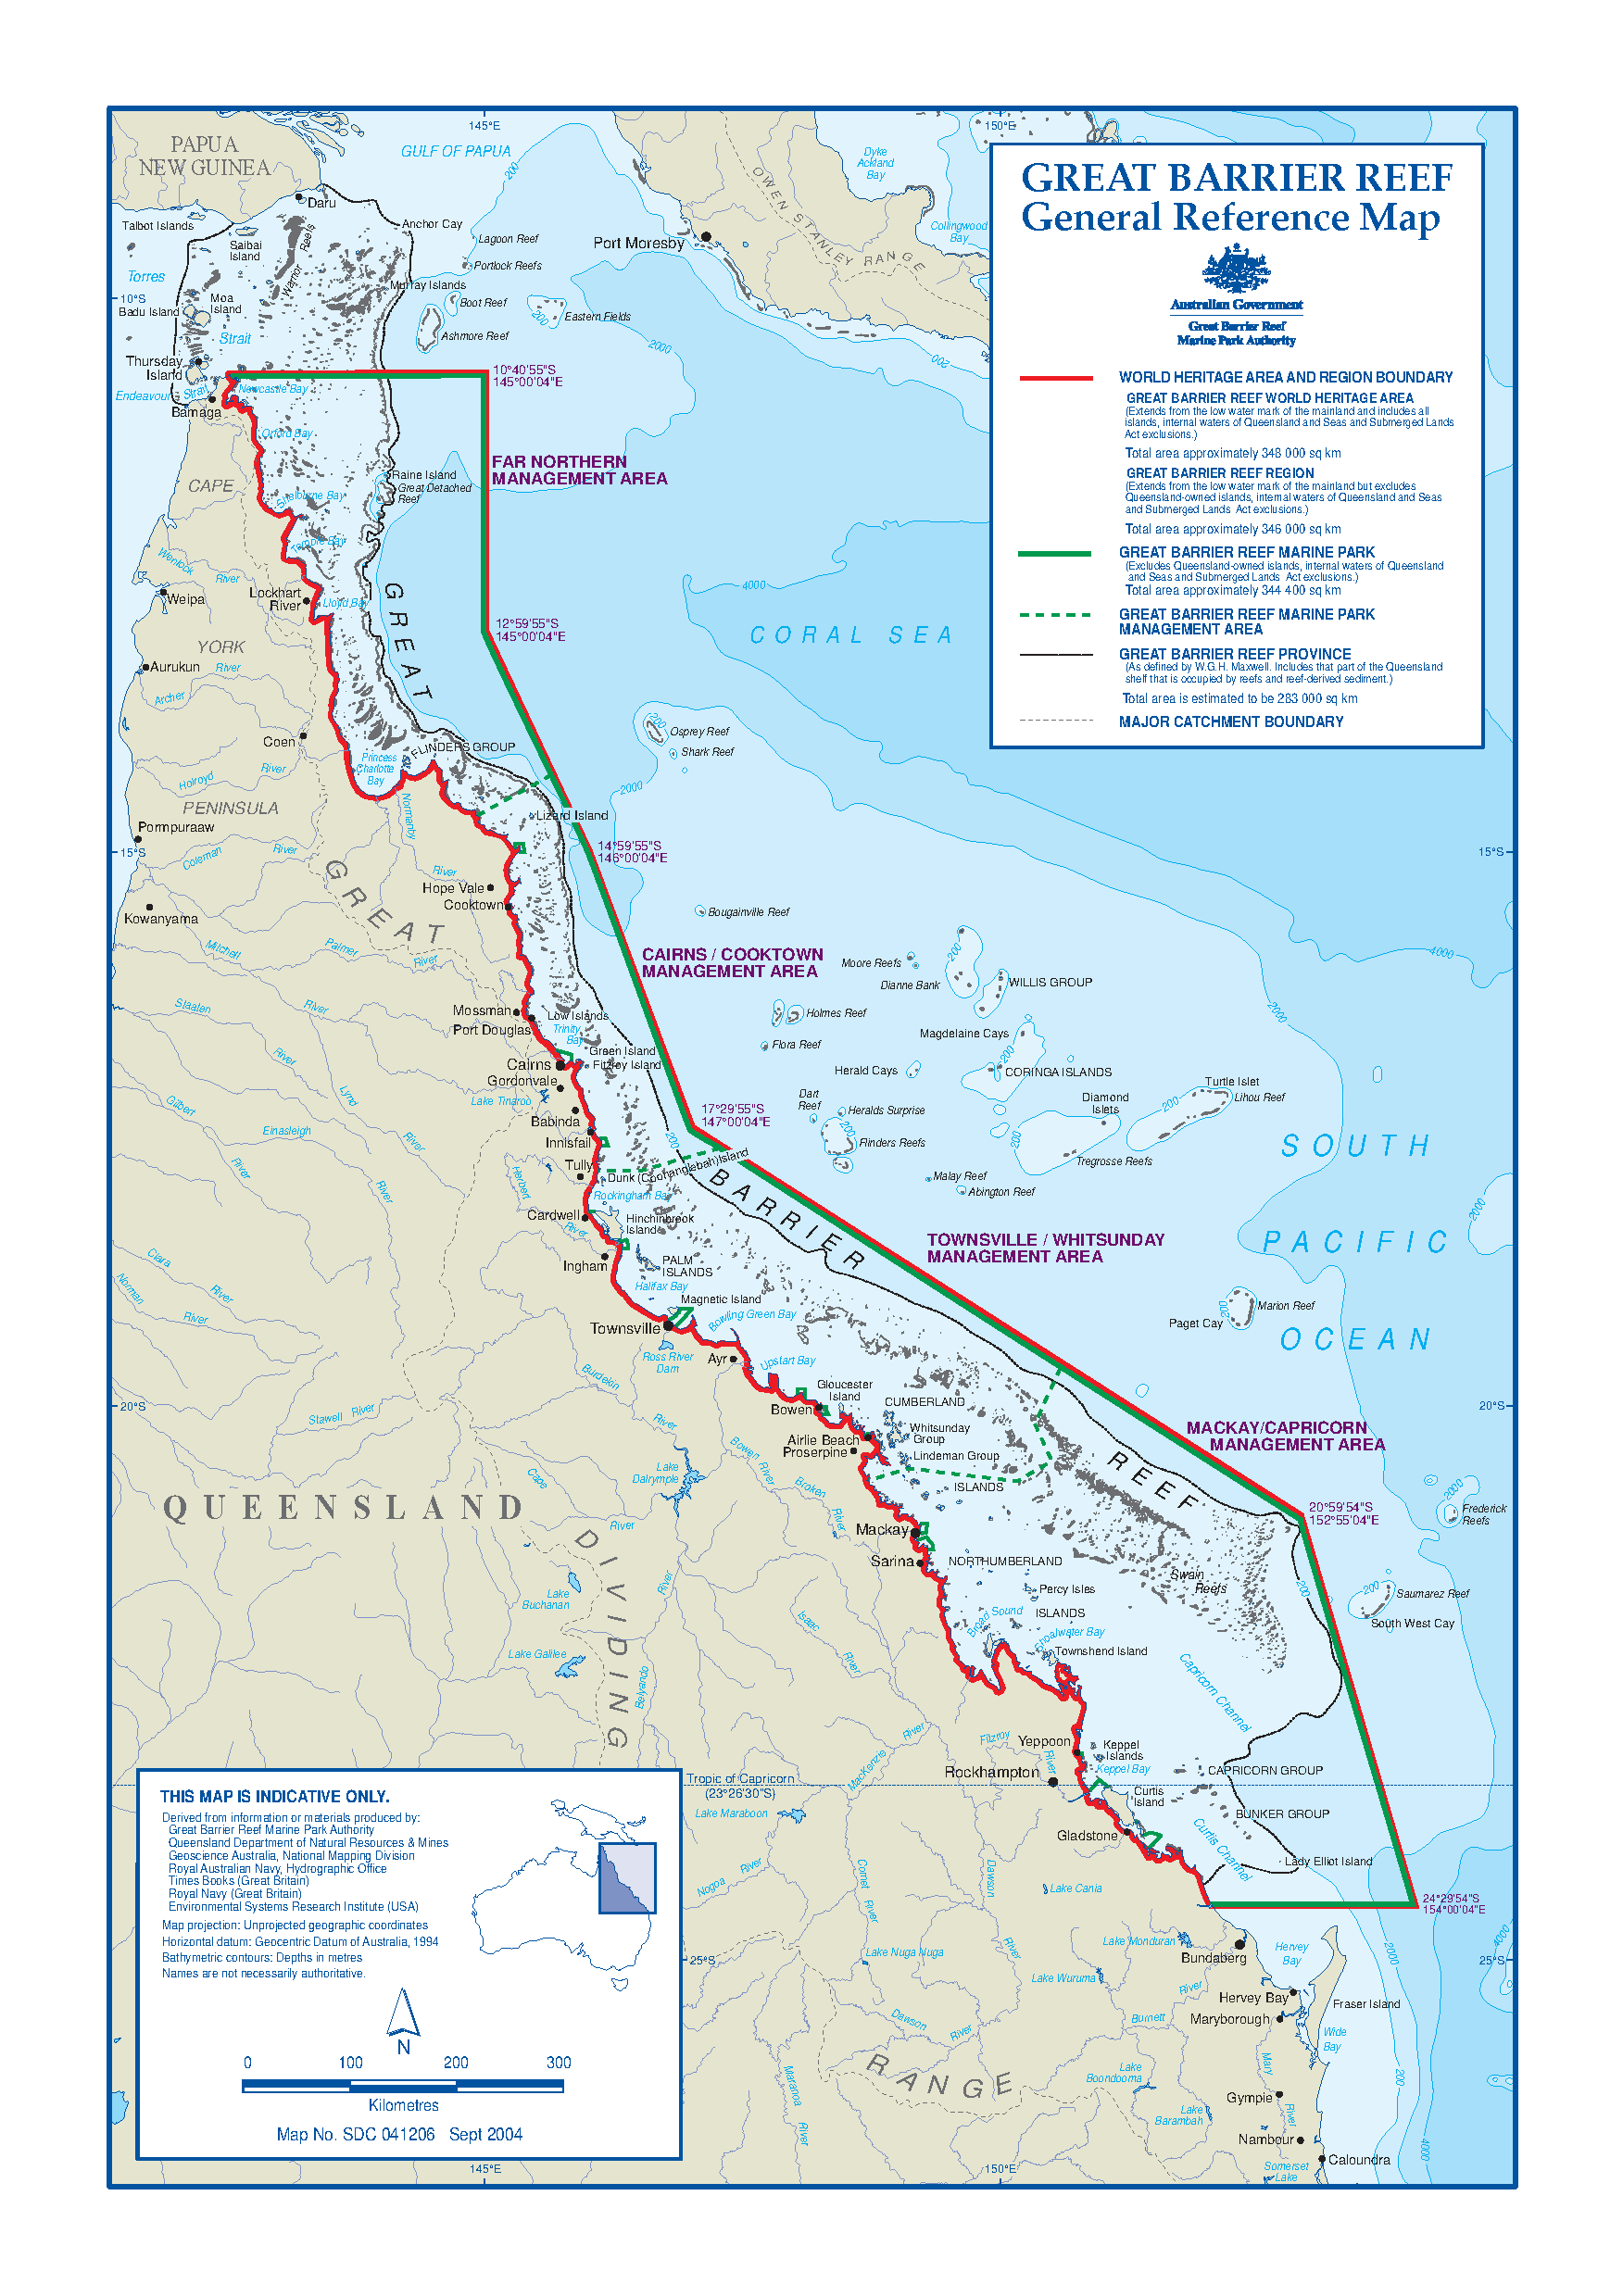
\includegraphics[width=0.9\textwidth,natwidth=787,natheight=1135]{Fig/GBR_map.pdf}
	    \caption{The boundary of the Great Barrier Reef Marine Park illustrating the extent of its coverage along the Queensland coast \citep{borthwick:2006uv}.}
	    \label{fig:gbrboundary}
	\end{figure}

	Climate change is causing an increase in sea surface temperature (\gls{sst}), which effects coral survival in the \gls{gbr} \citep{hoeghguldberg:1999bi}. Most corals rely on a symbiotic relationship with algae for energy, but when sufficiently stressed, the algae is ejected, this is coral bleaching \citep{hoeghguldberg:1999bi}. Stresses associated with changing conditions, and bleaching events, may also impact coral's production of \gls{dms} \citep{raina:2013fj}.

	Satellite imagery has been used to try and establish a link between \gls{sst} and cloud coverage in the \gls{gbr}. \citet{leahy:2013en} found relationships where changes in \gls{sst} was responsible for changes in cloud cover, but also that cloud cover was responsible for changes in \gls{sst}. Both were found to have a three day delay. The \gls{sst} to cloud cover correlation implies a negative feedback mechanism for cloud formation, with \gls{dms} produced by stressed coral mentioned as a possible source \citep{leahy:2013en}.

%------------------------------------------------------------------------------------------------------------------
%------------------------------------------------------------------------------------------------------------------

	\section{Coral DMS Production}
	\label{subsec:coraldms}

	While the \gls{claw} hypothesis was based only on phytoplankton as a producer of \gls{dms}, phytoplankton are not the only organisms responsible for its production. \gls{dmsp} production by coral is another source. Research has been performed on the effects of ocean temperature changes \citep{jones2007factors}, and the role of Symbiodinium (the algae that lives inside coral in a symbiotic relationship) in \gls{dmsp} production \citep{raina:2013fj}. \gls{dmsp} is converted to \gls{dms} by bacteria in the ocean \citep{todd2007structural}.

	Separate research on \gls{dmsp} production by Symbiodinium, and adult coral, had previously shown a discrepancy in total \gls{dmsp} production. Experimentation on the larval phase of coral yet to be inhabited by Symbiodinium has shown that coral larvae produce \gls{dmsp} independently \citep{raina:2013fj}. \gls{dmsp} concentration from coral was also found to be two times higher than that produced by benthic algae common to the \gls{gbr} \citep{raina:2013fj}. 

	%Coral was raised in the dark and DNA marker tests were used to rule out the presence of Symbiodinium or other algae. NMR was used to observe \gls{dmsp} concentration. \gls{dmsp} concentration was found to be two times higher than that produced by benthic algae common to the \gls{gbr}. The concentration also increased over time ruling out any carry over effect.

	An increase in temperature has been found to result in an increase in coral \gls{dmsp} production (see \cref{fig:coralstressdms}). \gls{dms} is known to have antioxidative effects, implying that increased \gls{dmsp} production is a defence against damage caused by heat stress. Adult colonies whose Symbiodinium was destroyed by heat stress also produced increasing levels of \gls{dmsp} with increasing temperatures. Prior to \citet{raina:2013fj}, it was assumed that increasing temperatures killing off the Symbiodinium would quickly decrease \gls{dmsp} production. This no longer appears to be the case.

	\begin{figure}[!htb]
	 	\centering
	    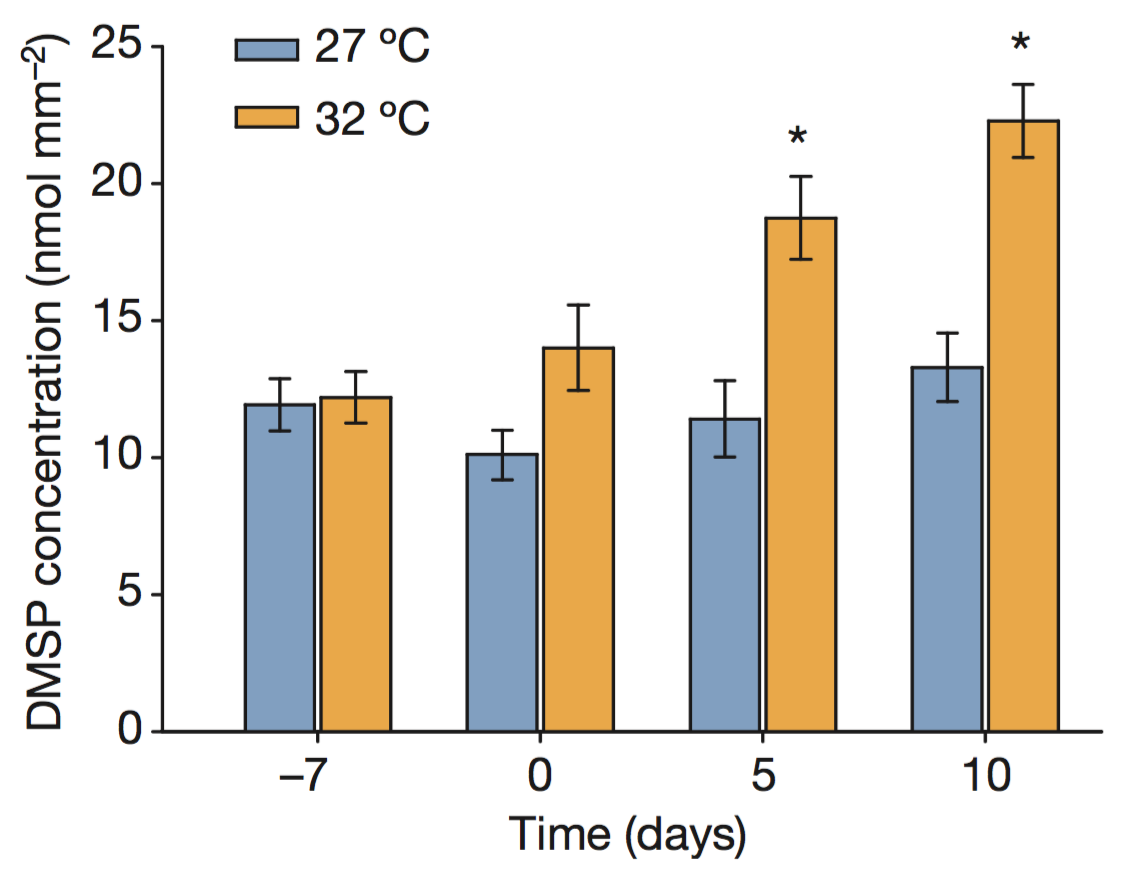
\includegraphics[width=0.7\textwidth,natwidth=1122,natheight=888]{Fig/coraldmspconcvstemp.png}
	    \caption{Adult coral \gls{dmsp} production increases when stressed by a higher temperature over an extended time period \citep{raina:2013fj}.}
	    \label{fig:coralstressdms}
	\end{figure}

	If \gls{dmsp} concentration has a resulting effect on cloud formation through \gls{ccn}, changing coral cover due to changing climate may impact local climate regulation.

	% As the original version of the \gls{claw} hypothesis did not include coral as a producer of \gls{dms}, coral's ability to influence climate was not considered. The temperature and stress dependance of coral \gls{dms} production satisfies the basic requirements of the production mechanism needed for \gls{claw}, but with a constant presence, unlike the blooms of phytoplankton species \cite{Charlson:1987fw}. 


%------------------------------------------------------------------------------------------------------------------
%------------------------------------------------------------------------------------------------------------------

 \section{GBR DMS Production}
 \label{sec:gbrdms}

 	Coral's eventual production of \gls{dms} in the \gls{gbr} region has been explored experimentally. Results from the \gls{gbr} indicate that corals can produce very high concentrations of \gls{dms} and \gls{dmsp} \citep{broadbent2004dms}. These concentrations also appear to depend on \gls{sst}s, and on tidal levels \citep{jones2007factors}. The extent of the \gls{gbr} presents a large source of sulphur that enters the atmosphere \citep{jones:2005ez}. 

 	The \gls{gbr} region is exposed regularly to south-easterly and southerly trade winds, providing the wind shear required to transfer \gls{dms} from the ocean to the atmosphere \citep{liss:1983iu}. During a voyage in $1997$, \citet{jones:2005ez} measured the highest levels of atmospheric \gls{dms} when these trade winds passed over large areas of the reef experiencing low tides (see \cref{fig:dmslowtide}). 

	\begin{figure}[!htb]
	 	\centering
	    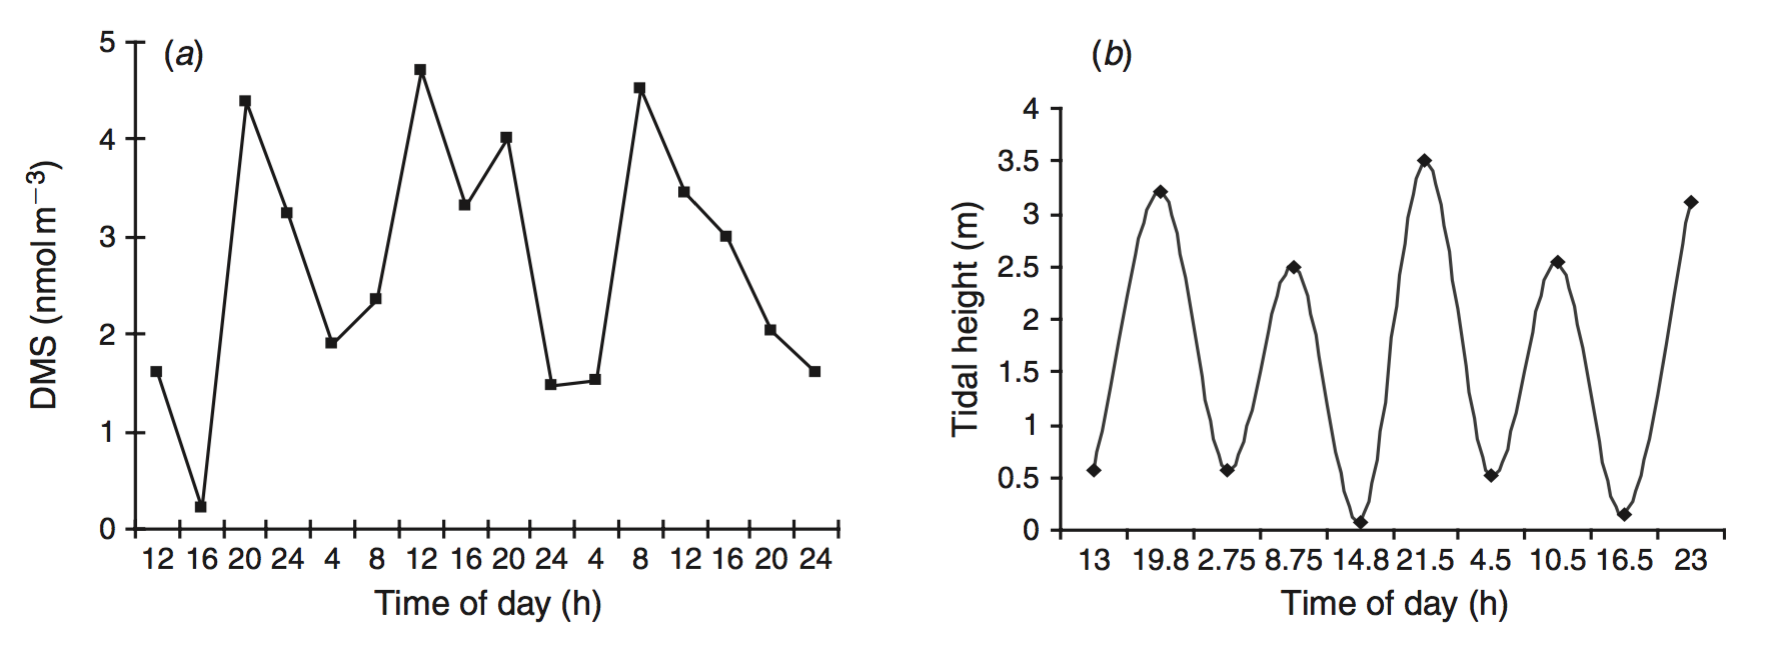
\includegraphics[width=0.9\textwidth,natwidth=1782,natheight=664]{Fig/DMS_tidal_link.png}
	    \caption{Data indicating the presence of a delayed link between atmospheric \gls{dms} concentrations and low tide events in the northern \gls{gbr} and NW Coral Sea \citep{jones:2005ez}.}
	    \label{fig:dmslowtide}
	\end{figure}

 	From here the production of \gls{ccn} from \gls{gbr} sourced \gls{dms} is not as well established. Much depends on the meteorology of the region and the relative concentrations of competing \gls{ccn} and \gls{dms} sinks. Localised modelling is needed to provide predictions in this area of research \citep{cainey:2007jj}.

 	
